\documentclass[english]{article}
\setlength{\parindent}{0pt}
\usepackage[paper=a4paper,layout=letterpaper]{geometry}
\usepackage[utf8]{inputenc}
\usepackage[english]{babel}
\usepackage{float}
\usepackage{physics,amssymb}
\usepackage{graphicx}
\usepackage{xcolor}   
\usepackage{tikz}            
\usepackage{subfigure}
\usepackage{amsmath}
\usepackage{amsbsy}
\usepackage{enumitem}

% For å lage referanser
\usepackage[
backend=biber,
style=verbose,
sorting=ynt
]{biblatex}
\addbibresource{Project1/referanser.bib}

% For å lage hyperlenker
\usepackage{hyperref}
\hypersetup{
    colorlinks,
    linkcolor={red!50!black},
    citecolor={blue!50!black},
    urlcolor={blue!80!black}}

% For å legge ved kode e.l.
\usepackage{listings}
\lstset{
	inputpath=,
	backgroundcolor=\color{white!88!black},
	basicstyle={\ttfamily\scriptsize},
	commentstyle=\color{magenta},
	language=Python,
	morekeywords={True,False},
	tabsize=4,
	stringstyle=\color{green!55!black},
	frame=single,
	keywordstyle=\color{blue},
	showstringspaces=false,
	columns=fullflexible,
	keepspaces=true}
	
	
% Kommandoer
\renewcommand{\d}{\mathrm{d}} % ikke-skråstilt infinitessimal
\renewcommand{\vec}{\mathbf} % bruke bold-vektorer heller enn piler
\newcommand{\vecsym}{\boldsymbol} % bold-vektor for greske bokstaver og symboler


\begin{document}
\title{Solving the Poisson equation in 1D} 
\author{Carl Martin Fevang, Håkon Kvernmoen}   
\date{\today}    

\maketitle
\abstract{We solved the 1D Poisson equation using Dirichlet boundary conditions on a charge density following $f(x) = 100e^{-10x}$}. We used a matrix representation of the double derivative and solved the set of linear equations with 3 different algorithms. First using an LU-decomposition with $2/3 n^3$ FLOPs where $h=10^{-1}, 10^{-2}, 10^{-3}$. Then with the Thomas algorithm using $8n$ FLOPs and finally a special case of the Thomas algorithm with known values on the diagonals reducing the FLOPs to $4n$ (both with $h=10
^{-1}$ to $h = 10^{-7}$). Using an analytical solution we analyzed the error over different step lengths and found that the optimal step length should be between $10^{-6}$ and $10^{-5}$.

\section{Introduction}
 In this report we are going to look at some simple numerical methods for solving the Poisson equation in one dimension. This equation is omnipresent in physics, and will often yield differential equations without any analytical solutions. The accuracy of our numerical procedures of solving are therefore obvious targets for examination. We will solve a rather simple version of the equation, with Dirichlet boundary conditions, using approximations for the second derivative and linear algebra. This allows us to examine how the granularity of our numerical procedures affects the precision of our solution, when compared to the analytical solution. Our goal is to quantitatively point to what kind of errors occur when implementing numerical methods on a computer, and to what extent.

The time complexity of an algorithm is also crucial and we will run the algorithms many times to approximate the mean time for each algorithm at different step lengths. Comparing the results we can quantitative compare the different algorithms.
\section{Theory}
\subsection{Poisson's equation}
Generally Poisson's equation\autocite{Poisson} is written as
\begin{align*}
    \nabla^2 \phi = f
\end{align*}
for a given function $f$ and an unknown function $\phi$. In electrostatics, Gauss's law\autocite{Gauss} takes the form of Poisson's equation with $\Phi$ as the electric potential and $\rho(r)$ being the charge density as a function of $r$ in a spherically symmetric system:
\begin{align*}
    -\nabla^2 \Phi &= \frac{\rho(r)}{\epsilon_0} \\
    -\frac{1}{r^2} \frac{\d}{\d r}\Big( r^2\frac{\d \Phi}{\d r} \Big) &= \frac{\rho(r)}{\epsilon_0}
\end{align*}
Using the substitution $\Phi(r) = \phi(r)/r \Rightarrow \frac{\d \Phi}{\d r} = \frac{1}{r}\frac{\d \phi}{\d r} - \phi/r^2$ we get
\begin{align*}
    -\frac{1}{r^2} \frac{\d}{\d r}\Big( r\frac{\d \phi}{\d r} - \phi \Big) &= \frac{\rho(r)}{\epsilon_0} \nonumber \\
    -\frac{1}{r}\frac{\d^2 \phi}{\d r^2} &= \frac{\rho(r)}{\epsilon_0} \nonumber \\
    -\frac{\d^2 \phi}{\d r^2} &= \frac{r \rho(r)}{\epsilon_0}
\end{align*}

With a quick change of variables we get the following
\begin{align} \label{eq:problem}
    -\frac{\d^2 u}{\d x^2} &= f(x)
\end{align}
This way the three-dimensional system can be solved as a Poisson equation in a single dimension.

For this specific report,we will examin a Poisson equation of this format, with a right hand side $f(x) = 100e^{-10x}$ and with Dirichlet boundary conditions $u(0) = u(1) = 0$. Solving equation \eqref{eq:problem}, we get:
\begin{align*}
    -\frac{\d^2 u}{\d x^2} &= 100e^{-10x} \\
    -\d^2u &= 100e^{-10x} \,\d x^2 \\
   -u &= e^{-10x} + c_1x + c_2 \\
   u &= -e^{-10x} - c_1x - c_2
\end{align*}
Using the boundary conditions, we get:
\begin{align*}
    u(0) = -1 - c_2 &= 0 \\
    c_2 &= -1 \\
    \\
    \Rightarrow u(1) = -e^{10} - c_1 + 1 &= 0 \\
    c_2 &= 1 - e^{-10}
\end{align*}
So our analytical solution is then
\begin{align} \label{eq:analytical_solution}
    u(x) &= 1 - (1-e^{-10})x - e^{-10x}
\end{align}

\subsection{Numerical discretization}
When we solve problems numerically we can't use continuous variables as we normally do in mathematics. For the variable $x$ we can only operate with discrete values such $x_0, x_1, x_2 ... x_n$ where $x_i \in [x_0, x_n]$. For the function $f(x)$ we can project values $f_1, f_2, ... f_n$ such that $f_i = f(x_i)$. Similar projections can be done for all variables.

Because the need for discretization in a computer, infinitesimal differences, such as in differentiation, cannot be computed accurately. From the definition of the derivative, however, we can get an approximation. The first derivative of an arbitrary function $f(x)$ is defined accordingly
\begin{align*}
    \frac{\d f(x)}{\d x} &= \lim_{h \to 0}\frac{f(x+h)-f(x)}{h} \\
    &\Downarrow \\
    \frac{\d f(x)}{\d x} &\approx \frac{f(x+h)-f(x)}{h}
\end{align*}
Using our discretized variable $x_i$ and letting it be linearly space in the interval $[x_0, x_n]$ such that $x_i = x_0 + ih$, we get a discretized approximation for the derivative
\begin{align} \label{eq:num_diff}
    \frac{\d f_i}{\d x} \approx \frac{f_{i+1}-f_i}{h}
\end{align}
This introduces a mathematical error, that grows with the step size $h$.

Defining a function $g(x) = \frac{\d f(x)}{\d x}$, we can find the second derivative of $f(x)$ as $\frac{\d g(x)}{\d x}$. Using equation \eqref{eq:num_diff}, we can thereby get an approximation for the second derivative:
\begin{align} \label{eq:2nd_num_diff}
    \frac{\d^2 f_i}{\d x^2} \approx \frac{f_{i+1}+f_{i-1}-2f_i}{h^2}
\end{align}
This leaves a numerical error that follows $h^2$.

Combining the approximation \eqref{eq:2nd_num_diff} and equation \eqref{eq:problem}, we get a discretized variant
\begin{align}
    \frac{u_{i+1}+2u_i-u_{i-1}}{h^2} &= f_i
\end{align}



\subsection{Some linear algebra}
The above discretization of our differential equation can be written as a matrix equation, allowing us to use some manipulations from linear algebra. The equation reads
\begin{align*}
    \vec{Au} &= \vec{b}
\end{align*}
where $\vec{A}$ is an $n\times n$ matrix where the diagonal elements equal $2$ and the elements above and below the diagonal are $-1$. $\vec{u}$ is a vector of length $n$ and contains the unknown solution to our problem, and $b$ is a vector of length $n$ that contains the known right hand side function values multiplied by the step size $h$ as $h^2f(x_0), ..., h^2f(x_n)$. The solution can be optained with straight Gaussian elimination, but we will look at some better implementations to reduce computation time. 

As long as the equation is solvable, we know that $\vec{A}$ must be an invertible matrix. Furthermore, the matrix can be broken up into a lower triangular matrix $\vec{L}$ and an upper triangular matrix $\vec{U}$ such that $\vec{A} = \vec{LU}$. This is called a LU-decomposition. Using this allows us to break up the equation into two parts that are easier to solve due to the properties of $\vec{L}$ and $\vec{U}$:
\begin{align*}
    \vec{Ly} &= \vec{b} \\
    \vec{Uu} &= \vec{y}
\end{align*}




\section{Implementation}
All the programs (algorithms, plotting and benchmarking) are available at \url{https://github.com/haakonkvernmoen/FYS3150}

We will use three algorithms, each more specific for our problem. The first algorithm we will use to solve our Poisson equation for $n$ equally space integration points is an LU decomposition. This algorithm requires the use of $n\times n$-matrices, and as such is both computationally heavy and cumbersome on memory. Further, we will show that our discretized Poisson equation leads to a tridiagonal matrix that we can solve using the Thomas algorithm. This algorithm will only use vectors of length $n$ and should be must quicker and more wieldy than the LU decomposition. Lastly, we will make some further simplifications to this algorithm, using some properties of the matrix specific to our problem.

The matrices and vectors we use have dimensions of $n \times n$ and $n$ respectively. Since we are using Dirichlet boundary conditions $u(0) = 0$ and $u(1) = 0$ are not included in the matrices/vectors (they are known). This leaves us with a total of $n+2$ points and a step length of $h = 1/(n+1)$. 

We will examine the relative error of this last algorithm compared with the analytic solution as a function of the step-size $h$. Lastly, the algorithms will be timed and comparisons will be made to examine the efficiency of the algorithms in practice. 

\subsection{LU decomposition}
To find the LU decomposition of our matrix $\vec{A}$, we will us the Doolittle algorithm. Our matrix $\vec{A}$ can be broken down as follows
\begin{equation*}
\begin{pmatrix}
a_{11} & a_{12} & \cdots & a_{1n} \\
a_{21} & a_{22} & \cdots & a_{2n} \\
\vdots  & \vdots  & \ddots & \vdots  \\
a_{n1} & a_{n2} & \cdots & a_{nn} 
\end{pmatrix} =  \begin{pmatrix}
l_{11} & 0 & \cdots & 0 \\
l_{21} & l_{22} & \cdots & 0 \\
\vdots  & \vdots  & \ddots & \vdots  \\
l_{n1} & l_{n2} & \cdots & l_{nn} 
\end{pmatrix} \begin{pmatrix}
u_{11} & u_{12} & \cdots & u_{1n} \\
0 & u_{22} & \cdots & u_{2n} \\
\vdots  & \vdots  & \ddots & \vdots  \\
0 & 0 & \cdots & u_{nn} 
\end{pmatrix} 
\end{equation*}
Writing out the multiplication we obtain an expression for the $a_{ij}$ element of the matrix $\vec{A}$. 

\begin{equation}
    a_{ij} = \sum_{s = 1}^{n} l_{is}u_{sj}  
\label{eq:LU_gen}
\end{equation}
We know that for $s > i \Rightarrow l_{is} = 0$ and for $s > j \Rightarrow u_{sj} = 0$. This implies that we can construct $\vec{U}$ row-by-row and $\vec{L}$ column-by-column. From this we can get the entries for the first row of $u$'s and first column of $l$'s with the use of the expression \ref{eq:LU_gen}.

\begin{align*}
    a_{1j} &= \sum_{s=1}^{1} l_{1s} u_{sj} = l_{11} u_{1j} \Rightarrow u_{1j} = \frac{a_{1j}}{l_{11}} \hspace{10px} j = 1, 2, ... , n \\
    a_{i1} &= \sum_{s=1}^{1} l_{is}u_{s1} = l_{i1}u_{11} \Rightarrow l_{i1} = \frac{a_{i1}}{u_{11}} \hspace{14px} i = 1, 2, ... , n
\end{align*}
Next we will find the $k$-th row for $\vec{U}$ and the $k$-th column for $\vec{L}$ assuming that we correctly found the $1, 2, ... , k-1$ row/column. Again using the expression \ref{eq:LU_gen} we find that

\begin{equation*}
    a_{kk} = \sum_{s=1}^{k} l_{ks}u_{sk} = \sum_{s=1}^{k-1} l_{ks}u_{sk} + l_{kk}u_{kk}
\end{equation*}
As we can see one of the diagonals $u_{kk}$ and $l_{kk}$ can be chosen rather arbitrary. From convention we will set $l_{kk} = 1$ and solve for $u_{kk}$. Finally we again use the expression \ref{eq:LU_gen} and find the $k$-th row of $\Vec{U}$ and the $k$-th column of $\Vec{L}$

\begin{align}
        a_{kj} &= \sum_{s=1}^{k} l_{ks}u_{sj} = \sum_{s=1}^{k-1} l_{ks}u_{sj} + l_{kk}u_{kj} \Rightarrow u_{kj} = a_{kj}- \sum_{s=1}^{k-1} l_{ks}u_{sj} \hspace{10px} j = k+1, ... , n \label{eq:LU_u}\\
        a_{ik} &= \sum_{s=1}^{k} l_{is}u_{sk} = \sum_{s=1}^{k-1} l_{is}u_{sk} + l_{ik}u_{kk} \Rightarrow  l_{ik} = \frac{a_{ik}-\sum\limits_{s=1}^{k-1} l_{is}u_{sk}}{u_{kk}} \hspace{10px} j = k+1, ... , n \label{eq:LU_l}
\end{align}
We can now iterate over the rows and columns and obtain the elements for the $\Vec{L}$ and $\Vec{U}$ matrices using expression \ref{eq:LU_l} and \ref{eq:LU_u} respectively. Note that since we forced $l_{kk} = 1$ there is no denominator in expression \ref{eq:LU_l} and we have to find the elements for $\Vec{U}$ before we find the elements for $\Vec{L}$. We also assume that $u_{kk} \neq 0$ to avoid division by zero errors. 


Although not straight forward to analyze, the number of FLOPs this algorithm requires is $\frac{2}{3}n^3$, ignoring the lower-order terms \autocite{LU_decomp}.



\subsection{Thomas algorithm}
The Thomas algorithm seeks to solve the same matrix equation $\vec{A}\vec{u}=\vec{b}$ as with the LU decomposition. However, when $\vec{A}$ is a tridiagonal matrix, some tricks can be implemented. A general tridiagonal $n\times n$ matrix can be written as
\begin{align*}
    \vec{A} &=
    \begin{pmatrix}
        d_1 & e_1 & 0 & \cdots & 0 \\
        c_1 & d_2 & e_2 & \cdots & 0 \\
        0 & c_2 & d_3 & \ddots & 0\\
        \vdots  & \vdots  & \ddots & \ddots & \vdots  \\
        0 & 0 & \cdots & c_{n-1} & d_n 
    \end{pmatrix}
\end{align*}
As we see here, the entire matrix can be defined through the vector $\vec{c}$, $\vec{d}$ and $\vec{e}$. We will use Gaussian elimination to get rid of the lower diagonal elements, which will introduce a new diagonal vector  $\vec{\Tilde{d}}$ and an altered right-hand-side vector $\vec{\Tilde{b}}$, where the elements are defined as:
\begin{align*}
    \Tilde{d}_i &= d_i - \frac{c_{i-1}e_{i-1}}{\Tilde{d}_{i-1}} \\
    \Tilde{b}_i &= b_i - \frac{c_{i-1}b_{i-1}}{\Tilde{d}_{i-1}}
\end{align*}
for $i = 2, ..., n$. Defining $q=c_{i-1}/\Tilde{d}_{i-1}$ we can skip one FLOP. The startpoints are unaltered as $\Tilde{d}_1 = d_1$ and $\Tilde{b}_1 = b_1$. This is the forwards substitution, and it leaves us with the matrix equation
\begin{align*}
    \begin{pmatrix}
        \Tilde{d}_1 & e_1 & 0 & \cdots & 0 \\
        0 & \Tilde{d}_2 & e_2 & \cdots & 0 \\
        0 & 0 & \Tilde{d}_3 & \ddots & 0 \\
        \vdots  & \vdots  & \ddots & \ddots & \vdots \\
        0 & 0 & \cdots & 0 & \Tilde{d}_n 
    \end{pmatrix}
    \begin{pmatrix}
        u_1 \\ u_2 \\ u_3 \\ \vdots \\ u_n
    \end{pmatrix}
    = 
    \begin{pmatrix}
        \Tilde{b}_1 \\ \Tilde{b}_2 \\ \Tilde{b}_3 \\ \vdots \\ \Tilde{b}_n
    \end{pmatrix}
\end{align*}

Again using Gaussian elimination, this time to rid ourselves of the upper diagonal elements of our altered matrix $A$, we obtain the solution for $\vec{u}$ as
\begin{align*}
    u_i &= \frac{\Tilde{b}_i - e_i u_{i+1}}{\Tilde{d}_i}
\end{align*}
for $i = n-1, n-2, ..., 1$. This part of the algorithm is the backwards substitution.

Counting the number of floating point operations required using this algorithm, we can see that there are $5(n-1)$ operations for the forward substitution and $3(n-1)$ for the backwards one, for a total of $8n$, as $n$ grows large.



\subsection{Thomas algorithm for singularly valued diagonals}
For a tridiagonal matrix where all the elements of the three diagonal vectors $\vec{c}$, $\vec{d}$, $\vec{e}$ are respectively the same, we can make some simplifications. In our case $\vec{c} = \vec{e} = (-1, -1, ..., -1)$, and $\vec{d} = (2, 2, ..., 2)$. Plugging these values into the forward substitution of the Thomas algorithm gives us a recursive formula for $\Tilde{d}_i$
\begin{align*}
    \Tilde{d}_i = 2 - \frac{1}{\Tilde{d}_{i-1}}
\end{align*}
which is a difference equation, the solution of which is
\begin{align*}
    \Tilde{d}_i &= \frac{i+1}{i}
\end{align*}
This result can just be plugged in, together with the value for $\vec{c}$, into the equation for $\Tilde{b}_i$:
\begin{align*}
    \Tilde{b}_i &= b_i + \frac{b_{i-1}}{\Tilde{d}_{i-1}}
\end{align*}
This means we get analytical solutions for the coefficients of the backwards substitution of the algorithm:
\begin{align*}
    u_i = \frac{\Tilde{b}_i + u_{i+1}}{\Tilde{d}_{i}}
\end{align*}

These simplifications allows us to vectorize the computation of the coefficients and improve the time it takes to execute the substitutions on a computer.

Counting the number of floating point operations now, we can ignore the vectorizable coefficients, and we have simply $2(n-1)$ operations for the forward substitution and $2(n-1)$ for the backwards one, for a total of $4n$ operation for large values of $n$.

\subsection{Benchmarking}

How fast a computer can run an algorithm depends on many factors, and simply doing one run for each algorithm at different step lengths $h$ is not very precise. Therefore we wrote a program that iterates over each algorithm and each step length $N=200$ times. Using the mean of all these values and the standard deviation as an uncertainty we can calculate the experimental time complexities. For the algorithm using LU decomposition we will time the actual LU decomposition, the forward substitution and the backward substitution for $h=10^{-1}$ to $10^{-3}$. For the Thomas algorithm we will time the backward and forward substitution for $h= 10
^{-1}$ to $h = 10^{-7}$. When using the Thomas algorithm with singular valued diagonals the calculations for the reduced diagonal elements $\Tilde{d}_i$ can be vectorized and we will only time the calculations for $\Tilde{b}_i$ and the backward substitution.    

\section{Results}
The results of the numerical solution follow the analytical solution closely. For our simplified Thomas algorithm the numerical solutions for various step sizes are superimposed on the analytical solution in figure \ref{fig:num_sol}.
\begin{figure} [H]
    \centering
    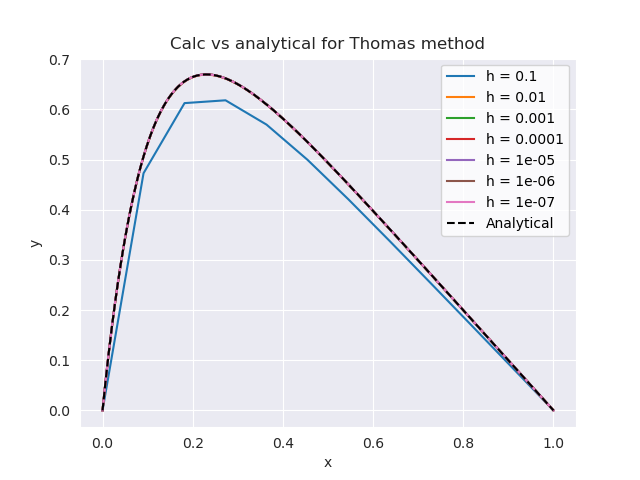
\includegraphics[width=8cm]{Project1/figurer/numerical_solution.png}
    \caption{The numerical solution of $\frac{\d^2 u}{\d x^2} = 100e^{-10x}$ for step sizes $h=10^{-1}, ..., 10^{-7}$.}
    \label{fig:num_sol}
\end{figure}
The maximum relative error in any integration point is plotted in figure \ref{fig:num_err}. A linear regression was also fitted over the points that seemed to follow the mathematical error. This returned a slope of $1.98$, with a standard deviation $0.01$.
\begin{figure} [H]
    \centering
    \includegraphics[width=8cm]{Project1/figurer/numerical_erros.png}
    \caption{The maximum relative error of any point of the numerical solutions as a function of the step size $h$. Using logarithmic scale on both axes.}
    \label{fig:num_err}
\end{figure}

Timing of the various algorithms $200$ times each with for $n=1, 2, ..., 7$ provided the results in figure \ref{fig:time}.
\begin{figure} [H]
    \centering
    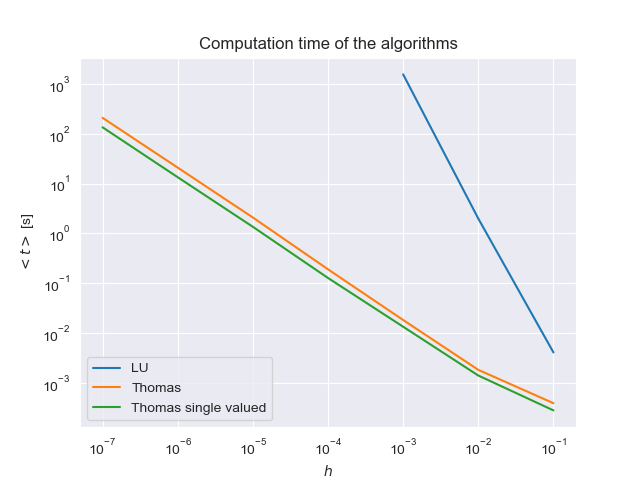
\includegraphics[width=8cm]{Project1/figurer/time.png}
    \caption{The time it took to compute the numerical solution of the Poisson equation using LU decomposition, the Thomas algorithm, and our simplified Thomas algorithm with error bars. }
    \label{fig:time}
\end{figure}
When timing the different algorithms we ran the LU decomposition with $n = 10, 100$ and $1000$ points. Both the Thomas algorithm and Thomas algorithm for singularly valued diagonals was computed for $n = 10$ to $n = 10^7$ integration points. The results are presented in figure \ref{fig:time}. The LU decomposition is significantly slower than the two others and unsuitable for small step lengths. The two Thomas algorithms are closer in computational time, but our singular valued algorithm preforms consistently better than the other. 



\section{Discussion}
It is clear from figure \ref{fig:num_sol} that the numerical solutions follow the analytical one closely for step sizes of 0.01 and smaller. Figure \ref{fig:num_err} gives us a deeper analysis of the validity of our solutions. Already at $h=0.01$ the maximum relative error is of the order $10^{-3}$. The error evolves as we would have predicted mathematically for the until the step sizes grow smaller than $10^{-5}$. For this first part, our linear regression showed a slope of $1.98 \pm 0.01$, which goes to show that the numerical error seems to be $O(h^2)$. Later however, as $h$ gets smaller, we recognize a distinct ``hockey stick'' shape to the graph, as the error grows larger as the step size is decreased. This is due to the numbers that are used to compute the solution become sufficiently small that the truncation of the decimals becomes significant enough to have an effect on the precision of the result. Thus, it is important to see whether your numerical results could be affected by such errors. Running the algorithm  with more step lengths between $h=10
^{-5}$ and $h=10^{-6}$ could help us determine the optimal step length, but in this report we found that the optimal step length should be somewhere between these two values.

When counting FLOPs we only included the arithmetic operations +, -, *, / and assumed that all of these required the same amount of computation power (on the CPU) \autocite{FLOPs}. This is not true since the cheapest operations are addition and subtraction. Multiplication takes more than these two and division  is even worse. In our counting we assumed that all of these are equal which does not reflect reality. Operations like fetching an element from an array and inserting a value to an array also takes some computation power, but we neglect these as they are very small and the arithmetic operations overshadows them.   

In figure \ref{fig:time} we see that the two Thomas algorithms slope much less steeply than the LU-decomposition, which is consistent with their respective number of FLOPs. Furthermore, the refined Thomas algorithm is faster than the general one, as expected. We could only compute the result from the LU decomposition for $n=1,2,3$, since it requires $n\times n$ matrices to be stored in memory. Every entry of this matrix is a double float, requiring 8 bytes each, which results in a memory usage of $10^{5} \cdot 10^{5} \cdot 8 \approx 8$ GB of memory. Furthermore, if it takes $T_p$ time to compute the $3/2 \, 10^{3p}$ FLOPs required of the LU decomposition, it should take $T_{p+1} = 10^3 \cdot T_p$ time to compute for the next power of 10. From figure \ref{fig:time} we can see that for $p=3$ it takes more than a second to compute the LU decomposition, as such it will take at least more than 15 minutes to compute for $p=4$ and nearly two weeks to compute for $p=5$. We are on a deadline and do not have time for such tomfoolery.



\section{Concluding remarks}
We have now seen some of the considerations that need to be taken into account as we solve the one dimensional Poisson equation. The equation is an important one to solve in physics, and generally nice analytical solutions, such as the one we chose, are not available, and we need to resort to numerical approaches to find solutions.

The practical physicist requires two things from these numerical solutions; accuracy and efficiency. Using a simple approximation of the double derivative, we have achieved good accuracy from our solutions, as can be seen in figures \ref{fig:num_sol} and \ref{fig:num_err}. However, as we mitigate the mathematical error, a computational error creeps in, and we cannot achieve arbitrary accuracy. Our approximation of the second derivative was shown to be proportional to $h^{1.98 \pm 0.01}$, until the truncation error took over.

The algorithms performed differently in terms of efficiency. The LU decomposition was taxing both in therms of computation time and memory usage, although it still produced correct results. The Thomas algorithm, however, was astounding, as it reduced to problem to only require a number of operations proportional to $n$. This allows us to decrease the step size without sacrificing much in terms of efficiency. We could even simplify the general Thomas algorithm to fit our specific one, to create a slightly faster algorithm, as seen in figure \ref{fig:time}.

Thus it is quite possible to achieve both fast and accurate solution to the one-dimensional Poisson equation, using only simple approximations and some linear algebra. However, taking the specific problem into account, and being aware of the limitations of a computer, must be done in order to produce usable results.



\printbibliography


\end{document}
